% (find-LATEX "2020-2-C2-TFC.tex")
% (defun c () (interactive) (find-LATEXsh "lualatex -record 2020-2-C2-TFC.tex" :end))
% (defun C () (interactive) (find-LATEXsh "lualatex 2020-2-C2-TFC.tex" "Success!!!"))
% (defun D () (interactive) (find-pdf-page      "~/LATEX/2020-2-C2-TFC.pdf"))
% (defun d () (interactive) (find-pdftools-page "~/LATEX/2020-2-C2-TFC.pdf"))
% (defun e () (interactive) (find-LATEX "2020-2-C2-TFC.tex"))
% (defun o () (interactive) (find-LATEX "2020-2-C2-TFC.tex"))
% (defun u () (interactive) (find-latex-upload-links "2020-2-C2-TFC"))
% (defun v () (interactive) (find-2a '(e) '(d)))
% (defun d0 () (interactive) (find-ebuffer "2020-2-C2-TFC.pdf"))
% (defun cv () (interactive) (C) (ee-kill-this-buffer) (v) (g))
%          (code-eec-LATEX "2020-2-C2-TFC")
% (find-pdf-page   "~/LATEX/2020-2-C2-TFC.pdf")
% (find-sh0 "cp -v  ~/LATEX/2020-2-C2-TFC.pdf /tmp/")
% (find-sh0 "cp -v  ~/LATEX/2020-2-C2-TFC.pdf /tmp/pen/")
%     (find-xournalpp "/tmp/2020-2-C2-TFC.pdf")
%   file:///home/edrx/LATEX/2020-2-C2-TFC.pdf
%               file:///tmp/2020-2-C2-TFC.pdf
%           file:///tmp/pen/2020-2-C2-TFC.pdf
% http://angg.twu.net/LATEX/2020-2-C2-TFC.pdf
% (find-LATEX "2019.mk")
% (find-CN-aula-links "2020-2-C2-TFC" "2" "c2m202tfc" "c2t")
%
% Video:
% (find-ssr-links "c2m202tfc" "2020-2-C2-TFC")
% (code-video     "c2m202tfcvideo" "$S/http/angg.twu.net/eev-videos/2020-2-C2-TFC.mp4")
% (find-c2m202tfcvideo "0:00")

% «.defs»			(to "defs")
% «.subst-defs»			(to "subst-defs")
% «.title»			(to "title")
% «.exercicio-1»		(to "exercicio-1")
% «.exercicio-2»		(to "exercicio-2")
% «.integral-indefinida»	(to "integral-indefinida")
% «.int-subst-2»		(to "int-subst-2")
% «.exercicio-5»		(to "exercicio-5")
% «.exercicio-6»		(to "exercicio-6")
%
% «.djvuize»	(to "djvuize")

\documentclass[oneside,12pt]{article}
\usepackage[colorlinks,citecolor=DarkRed,urlcolor=DarkRed]{hyperref} % (find-es "tex" "hyperref")
\usepackage{amsmath}
\usepackage{amsfonts}
\usepackage{amssymb}
\usepackage{pict2e}
\usepackage[x11names,svgnames]{xcolor} % (find-es "tex" "xcolor")
\usepackage{colorweb}                  % (find-es "tex" "colorweb")
%\usepackage{tikz}
%
% (find-dn6 "preamble6.lua" "preamble0")
%\usepackage{proof}   % For derivation trees ("%:" lines)
%\input diagxy        % For 2D diagrams ("%D" lines)
%\xyoption{curve}     % For the ".curve=" feature in 2D diagrams
%
\usepackage{edrx15}               % (find-LATEX "edrx15.sty")
\input edrxaccents.tex            % (find-LATEX "edrxaccents.tex")
\input edrxchars.tex              % (find-LATEX "edrxchars.tex")
\input edrxheadfoot.tex           % (find-LATEX "edrxheadfoot.tex")
\input edrxgac2.tex               % (find-LATEX "edrxgac2.tex")
%
%\usepackage[backend=biber,
%   style=alphabetic]{biblatex}            % (find-es "tex" "biber")
%\addbibresource{catsem-slides.bib}        % (find-LATEX "catsem-slides.bib")
%
% (find-es "tex" "geometry")
\usepackage[a6paper, landscape,
            top=1.5cm, bottom=.25cm, left=1cm, right=1cm, includefoot
           ]{geometry}
%
\begin{document}

%\catcode`\^^J=10
%\directlua{dofile "dednat6load.lua"}  % (find-LATEX "dednat6load.lua")

% %L dofile "edrxtikz.lua"  -- (find-LATEX "edrxtikz.lua")
% %L dofile "edrxpict.lua"  -- (find-LATEX "edrxpict.lua")
% \pu

% «defs»  (to ".defs")
% (find-LATEX "edrx15.sty" "colors-2019")
\long\def\ColorRed   #1{{\color{Red1}#1}}
\long\def\ColorViolet#1{{\color{MagentaVioletLight}#1}}
\long\def\ColorViolet#1{{\color{Violet!50!black}#1}}
\long\def\ColorGreen #1{{\color{SpringDarkHard}#1}}
\long\def\ColorGreen #1{{\color{SpringGreenDark}#1}}
\long\def\ColorGreen #1{{\color{SpringGreen4}#1}}
\long\def\ColorGray  #1{{\color{GrayLight}#1}}
\long\def\ColorGray  #1{{\color{black!30!white}#1}}
\long\def\ColorBrown #1{{\color{Brown}#1}}
\long\def\ColorBrown #1{{\color{brown}#1}}
\long\def\ColorOrange#1{{\color{orange}#1}}

\long\def\ColorShort #1{{\color{SpringGreen4}#1}}
\long\def\ColorLong  #1{{\color{Red1}#1}}

\def\frown{\ensuremath{{=}{(}}}
\def\True {\mathbf{V}}
\def\False{\mathbf{F}}
\def\D    {\displaystyle}
\def\veq{\rotatebox{90}{$=$}}

\def\drafturl{http://angg.twu.net/LATEX/2020-2-C2.pdf}
\def\drafturl{http://angg.twu.net/2020.2-C2.html}
\def\draftfooter{\tiny \href{\drafturl}{\jobname{}} \ColorBrown{\shorttoday{} \hours}}


% «subst-defs»  (to ".subst-defs")
% (find-LATEX "2020-1-C2-TFC2-2.tex" "subst-defs")

\def\pfo#1{\ensuremath{\mathsf{[#1]}}}
\def\D{\displaystyle}

% Difference with mathstrut
\def\Difms #1#2#3{\left. \mathstrut #3 \right|_{s=#1}^{s=#2}}
\def\Difmu #1#2#3{\left. \mathstrut #3 \right|_{u=#1}^{u=#2}}
\def\Difmx #1#2#3{\left. \mathstrut #3 \right|_{x=#1}^{x=#2}}
\def\Difmth#1#2#3{\left. \mathstrut #3 \right|_{θ=#1}^{θ=#2}}

\def\iequationbox#1#2{
    \left(
    \begin{array}{rcl}
    \D{ #1 } &=& \D{ #2 } \\
    \end{array}
    \right)
  }
\def\isubstbox#1#2#3#4#5{{
    \def\veq{\rotatebox{90}{$=$}}
    \def\ph{\phantom}
    \left(
    \begin{array}{rcl}
    \D{ #1 } &=& \D{ #2 } \\
    {\veq#3} \\
    \D{ #4 } &=& \D{ #5 } \\
    \end{array}
    \right)
  }}
\def\isubstboxT#1#2#3#4#5#6{{
    \def\veq{\rotatebox{90}{$=$}}
    \def\ph{\phantom}
    \left(
    \begin{array}{rcl}
    \multicolumn{3}{l}{\text{#6}} \\%[5pt]
    \D{ #1 } &=& \D{ #2 } \\
    {\veq#3} \\
    \D{ #4 } &=& \D{ #5 } \\
    \end{array}
    \right)
  }}

% Definição das fórmulas para integração por substituição.
% Algumas são pmatrizes 3x3 usando isubstbox.

\def\TFCtwo{
  \iequationbox {\Intx{a}{b}{F'(x)}}
                {\Difmx{a}{b}{F(x)}}
}
\def\TFCtwoI{
  \iequationbox {\intx{F'(x)}}
                {F(x)}
}

\def\Sone{
  \isubstbox
    {\Difmx{a}{b}{f(g(x))}}  {\Intx{a}{b}{f'(g(x))g'(x)}}
    {\ph{mmm}}
    {\Difmu{g(a)}{g(b)}{f(u)}} {\Intu{g(a)}{g(b)}{f'(u)}}
}
\def\SoneI{
  \isubstbox
    {f(g(x))} {\intx{f'(g(x))g'(x)}}
    {\ph{m}}
    {f(u)}    {\intu{f'(u)}}
}

\def\Stwo{
  \isubstboxT
    {\Difmx{a}{b}{F(g(x))}}   {\Intx{a}{b}{f(g(x))g'(x)}}
    {\ph{mmm}}
    {\Difmu{g(a)}{g(b)}{F(u)}}  {\Intu{g(a)}{g(b)}{f(u)}}
    {Se $F'(u)=f(u)$ então:}
}
\def\StwoI{
  \isubstboxT
    {F(g(x))}  {\intx{f(g(x))g'(x)}}
    {\ph{m}}
    {F(u)}     {\intu{f(u)}}
    {Se $F'(u)=f(u)$ então:}
}

\def\Sthree{
  \iequationbox {\Intx{a}{b}{f(g(x))g'(x)}}
                {\Intu{g(a)}{g(b)}{f(u)}}
}
\def\SthreeI{
  \iequationbox {\intx{f(g(x))g'(x)}}
                {\intu{f(u)}
                 \qquad [u=g(x)]
                }
  % [u=g(x)]
}

\def\Sthree{
  \pmat{
    \D \Intx{a}{b}{f(g(x))g'(x)} \\
    \veq \\
    \D \Intu{g(a)}{g(b)}{f(u)}
  }}



%  _____ _ _   _                               
% |_   _(_) |_| | ___   _ __   __ _  __ _  ___ 
%   | | | | __| |/ _ \ | '_ \ / _` |/ _` |/ _ \
%   | | | | |_| |  __/ | |_) | (_| | (_| |  __/
%   |_| |_|\__|_|\___| | .__/ \__,_|\__, |\___|
%                      |_|          |___/      
%
% «title»  (to ".title")
% (c2m202tfcp 1 "title")
% (c2m202tfc    "title")

\thispagestyle{empty}

\begin{center}

\vspace*{1.2cm}

{\bf \Large Cálculo 2 - 2020.2}

\bsk

Aula 12: o TFC2.

\bsk

Eduardo Ochs - RCN/PURO/UFF

\url{http://angg.twu.net/2020.2-C2.html}

\end{center}

\newpage

\def\Rd{\ColorRed}

Na aula passada nós vimos esta versão do \ColorRed{segundo}

Teorema Fundamental do Cálculo:

% (c2m202escadasp 17 "primitivas-como-usar")
% (c2m202escadas     "primitivas-como-usar")

\begin{quote}

Se a função $F:[a,b]→\R$ é uma primitiva da função $f:[a,b]→\R$ e
$c,d∈[a,b]$, então:
%
$$\begin{array}{rcl}
  \D \Intx{c}{d}{f(x)} &=& \D \Difx{c}{d}{F(x)} \\
  \end{array}
$$

\end{quote}

A notação ``$\Difx{c}{d}{F(x)}$'' é novidade. A pronúncia de
``$\Difx{c}{d}{F(x)}$''

é ``a diferença do valor de $F(x)$ entre $x=c$ para $x=d$'',

e a definição formal é:
%
$$\begin{array}{rcl}
  \Difx{c}{d}{F(x)} &=& F(x)[x:=d] - F(x)[x:=c] \\
                    &=& F(d) - F(c). \\
  \end{array}
$$

\newpage

Nós não vimos uma \ColorRed{demostração} do TFC2... vimos só uns
argumentos que devem ter convencido vocês de que ele vale pra todas as
funções escada. As notas do Pierluigi têm um esboço da demonstração,
mas ele pula um monte de detalhes. A demonstração completa é bem
grande e não nos interessa neste curso --- nós queremos \Rd{usar} o
TFC2 pra calcular um monte de coisas.

Nesta aula e nas próximas nós vamos tratar o TFC2 como esta igualdade,
%
$$\pfo{TFC2} \;\;=\;\; \left( \D \Intx{c}{d}{F'(x)} = \Difx{c}{d}{F(x)} \right)$$
%
que vai valer para toda $F:[a,b]→\R$ derivável e para todos os
$c,d∈[a,b]$, e nós vamos usar a operação $[:=]$ para obter \Rd{casos
  particulares} desta fórmula.

(Sobre o TFC1: ele praticamente só serve pra demonstrar o TFC2...)


\newpage

Digamos que queremos ``integrar'' isto:
%
$$\Intx{3}{4}{e^{2x} \cos(e^{2x})} = \Rd{?}$$

\def\TFCDOIS#1#2#3#4{
  \pfo{TFC2} \subst{d:=#2 \\ c:=#1 \\ F(x):=#3 \\ F'(x):=#4}
  & = &
  \left(
  \D \Intx{#1}{#2}{#4} = \Difx{#1}{#2}{\left( #3 \right)}
  \right)
  }

Podemos usar o TFC2 várias vezes, chutando `$a$'s, `$b$'s e `$F$'s...

\msk

$\scalebox{0.80}{$
 \begin{array}{rcl}
  \TFCDOIS{42}{200}{\sen x}{\cos x} \\
  \TFCDOIS{3}{4} {        \sen(e^{2x})} {(2 e^{2x}) \cos(e^{2x}))} \\
  \TFCDOIS{3}{4} {\frac12 \sen(e^{2x})} {   e^{2x}  \cos(e^{2x}))} \\
  \end{array}
  $}
$

\bsk

Ou seja: $\Rd{?} = \Difx{3}{4}{\left( \frac12 \sen(e^{2x}) \right)}$,

que dá pra calcular \Rd{em tempo finito} --- se soubermos

calcular senos e exponenciais em tempo finito.

\newpage

% «exercicio-1»  (to ".exercicio-1")
% (c2m202tfcp 5 "exercicio-1")
% (c2m202tfc    "exercicio-1")

Vamos chamar o método do slide anterior de

``integração por TFC2 e chutar-e-testar''.

\msk

{\bf Exercício 1.}

Integre por TFC2 e chutar-e-testar:

\msk

a) $\D \Intx{0}{π/2}{\cos x} = \Rd{?}$

\msk

b) $\D \Intx{0}{π}{\sen x} = \Rd{?}$

\msk

c) $\D \Intx{π/2}{π}{\sen x} = \Rd{?}$

\msk

d) $\D \Intx{5}{6}{\sen(2x + 3)} = \Rd{?}$

\newpage

% «exercicio-2»  (to ".exercicio-2")

{\bf Exercício 2.}

Faça os 5 primeiros itens do Exercício 35 das notas do Pierluigi.

% (find-pierluigipage 13 "Exercício 35. Calcule as integrais seguintes:")
% (find-pierluigitext 13 "Exercício 35. Calcule as integrais seguintes:")

% f = x**2
% integrate(f, (x, 2, 3))
% f = 3*x + 5
% integrate(f, (x, 3, 4))



\newpage

% «integral-indefinida»  (to ".integral-indefinida")
% (c2m202tfcp 7 "integral-indefinida")
% (c2m202tfc    "integral-indefinida")
% (c2m201tfc22p 2 "integral-indefinida")
% (c2m201tfc22    "integral-indefinida")
% (find-martinscdipage (+ 10 109) "4.2.2       Integral Indefinida")
% (find-martinscditext (+ 10 109) "4.2.2       Integral Indefinida")

{\bf (Uma definição para) a integral indefinida}

Dê uma olhada na seção 4.2.2 do Martins/Martins.

Eles usam o ``$+ \; C$'' na definição de integral indefinida.

A maioria dos livros faz isso, mas isso gera algumas

ambiguidades que eu prefiro evitar...

\msk

Eu vou usar esta definição aqui para a integral indefinida.

As duas igualdades abaixo são \Rd{exatamente equivalentes}:
%
$$\begin{array}{ccr}
  \displaystyle \int {f(x)} \, dx &=& F(x) \\
                f(x)  &=& \frac{d}{dx} F(x) \\
  \end{array}
$$

Ou seja: pra determinar se uma igualdade da forma

``$\int {f(x)} \, dx \;=\; F(x)$'' é verdade, \Rd{traduza} ela, e teste se

a igualdade $f(x) \;=\; \frac{d}{dx} F(x)$ é verdade.


\newpage

{\bf Exercício 3.}

Quais das igualdades abaixo são verdade?

a) $\intx{\sen x} = \cos x$ 

b) $\intx{\cos x} = \sen x$ 

c) $\intx{x^4} = 5 x^5$ 

d) $\intx{x^4} = \frac15 x^5$ 

\ssk

e) $\intx{x^4} = \frac15 x^5 + 42$ 

\bsk

{\bf Exercício 4.}

As duas igualdades em
%
$$42 \;\;=\;\; \intx{0\,} \;\;=\;\; 200$$

são verdadeiras. Porque é que isto não implica em $42 = 200$?


\newpage

{\bf (Introdução à) integração por substituição}

Repare que estas duas integrais correspondem a áreas iguais:

(amasse os gráficos na horizontal e estique eles na vertical)

$$\begin{array}{rcl}
  \D \Intx{π/2}{π}{\sen x}
  &=&
  \Area\left(
  % (find-latexscan-links "C2" "20210316_sen_1")
  % (find-xpdf-page "~/LATEX/2020-2-C2/20210316_sen_1.pdf")
  \myvcenter{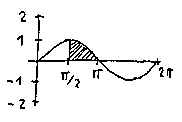
\includegraphics[height=2cm]{2020-2-C2/20210316_sen_1.pdf}}
  \right)
  \\
  \D \Intx{π/4}{π/2}{2 \sen 2x}
  &=&
  \Area\left(
  % (find-latexscan-links "C2" "20210316_sen_2")
  % (find-xpdf-page "~/LATEX/2020-2-C2/20210316_sen_2.pdf")
  \myvcenter{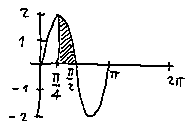
\includegraphics[height=2cm]{2020-2-C2/20210316_sen_2.pdf}}
  \right)
  \end{array}
  \\
$$

Vamos ver como \Rd{transformar} a segunda integral,

que é complicada, na primeira, que é mais simples.

\newpage

% «int-subst-2»  (to ".int-subst-2")
% (c2m201tfc22p 9 "S1")
% (c2m201tfc22    "S1")


{\bf (Introdução à) integração por substituição (2)}

Isto aqui é uma \Rd{demonstração} feita de uma

sequência de três igualdades, e um caso particular

dela...
%
$$\scalebox{0.8}{$
  \begin{array}[t]{rcl}
   \pfo{S1} &=& \Sone    \\
   %\pfo{S2} &=& \Stwo    \\
   \\
   \pfo{S1} \subst{g(x):=2x \\ g'(x):=2} &=&
     \isubstbox
      {\Difmx{a}{b}{f(2x)}}  {\Intx{a}{b}{f'(2x)·2}}
      {\ph{mmm}}
      {\Difmu{2a}{2b}{f(u)}} {\Intu{2a}{2b}{f'(u)}}
   \\
   %\pfo{S2} &=& \Stwo    \\
  \end{array}
  $}
$$




\newpage

% «exercicio-5»  (to ".exercicio-5")
% (c2m202tfcp 11 "exercicio-5")
% (c2m202tfc     "exercicio-5")

Lembre que:

$$\pfo{TFC2} \;\;=\;\; \left( \D \Intx{c}{d}{F'(x)} = \Difx{c}{d}{F(x)} \right)$$

\msk

{\bf Exercício 5.}

a) Qual é o resultado da substituição
   $\pfo{TFC2}
    \subst{
      d := b \\
      c := a \\
      F(x):=f(g(x)) \\
      F'(x):=f'(g(x))g'(x) \\
    }$ ?

b) Qual é o resultado de
   $\pfo{TFC2}
    [x:=u]
    \subst{
      d := g(b) \\
      c := g(a) \\
      F(u):=f(u) \\
      F'(u):=f'(u) \\
    }$ ?

c) Verifique que:
%
$$ \Difx{a}{b}{f(g(x))} = f(g(b)) - f(g(a)) = \Difu{g(a)}{g(b)}{f(u)} $$

d) Os itens (a), (b) e (c) provam as três igualdades da $\pfo{S1}$?


\newpage

% «exercicio-6»  (to ".exercicio-6")
% (c2m202tfcp 12 "exercicio-6")
% (c2m202tfc     "exercicio-6")

{\bf Exercício 6.}

No slide 9 eu disse, sem demonstração, que:
%
$$\Intx{π/2}{π}{\sen x}
  \;\;=\;\;
  \D \Intx{π/4}{π/2}{2 \sen 2x}
  \qquad
  (*)
$$

e no slide 10 a gente começou a transformar $\pfo{S1}$

numa demonstração de $(*)$.

Descubra o que colocar em cada um dos `\Rd{?}'s

abaixo para obter uma demonstração de $(*)$:
%
$$\pfo{S1}
  \subst{g(x):=2x \\ g'(x):=2}
  \subst{f(u):=\Rd{?} \\ f'(u):=\Rd{?}}
  \subst{b:=\Rd{?} \\ a:=\Rd{?}}
$$


%   \pfo{S1} \subst{g(x):=2x \\ g'(x):=2} &=&



\newpage

No slide 9 eu disse que a gente ia aprender a transformar

integrais mais complicadas em integrais mais simples.

No exercício 1d você deve ter passado um tempão

tentando resolver {\sl direto} uma integral complicada.

O truque é esse aqui. As $\pfo{S2}$ e $\pfo{S3}$ do próximo

slide são consequências da $\pfo{S1}$ do slide 10,

que você demonstrou no exercício 5...

\bsk

Dica {\bf MUITO} importante que {\bf MUITAS} pessoas

levam {\bf MUITO} tempo pra entender:

No item c do próximo slide você vai substituir a $f$

mas não a $F$, e a primeira linha da $\pfo{S2}$ vai

virar ``Se $F'(u) = \tan u$ então:''...




\newpage

$\scalebox{0.80}{$
 \begin{array}{rcc}
  \pfo{S2} &=& \Stwo \\
  \\
  \pfo{S3} &=& \Sthree \\
  \end{array}
 $}
$

\msk

{\bf Exercício 7.}

a) $\pfo{S3} \, [g(x):=x^2] = \Rd{?}$

b) $\pfo{S3} \, \subst{f(u):=\tan u \\ g(x):=x^2} = \Rd{?}$

c) $\pfo{S2} \, \subst{f(u):=\tan u \\ g(x):=x^2} = \Rd{?}$



% F = sin(exp(3*x))
% F = sin(exp(2*x)) / 2
% F.diff(x)


\newpage

$\scalebox{0.5}{$
  \begin{array}[t]{l}
   \pfo{S1} = \Sone    \\
  \\
  \pfo{S1}
  \subst{g(x):=2x \\ g'(x):=2}
  \subst{f(u):=\Rd{?} \\ f'(u):=\Rd{?}}
  \subst{b:=\Rd{?} \\ a:=\Rd{?}}
  \end{array}
  $}
$




\bsk







%\printbibliography

\GenericWarning{Success:}{Success!!!}  % Used by `M-x cv'

\end{document}

%  ____  _             _         
% |  _ \(_)_   ___   _(_)_______ 
% | | | | \ \ / / | | | |_  / _ \
% | |_| | |\ V /| |_| | |/ /  __/
% |____// | \_/  \__,_|_/___\___|
%     |__/                       
%
% «djvuize»  (to ".djvuize")
% (find-LATEXgrep "grep --color -nH --null -e djvuize 2020-1*.tex")

 (eepitch-shell)
 (eepitch-kill)
 (eepitch-shell)
# (find-fline "~/2020.2-C2/")
# (find-fline "~/LATEX/2020-2-C2/")
# (find-fline "~/bin/djvuize")

cd /tmp/
for i in *.jpg; do echo f $(basename $i .jpg); done

f () { rm -fv $1.png $1.pdf; djvuize $1.pdf }
f () { rm -fv $1.png $1.pdf; djvuize WHITEBOARDOPTS="-m 1.0" $1.pdf; xpdf $1.pdf }
f () { rm -fv $1.png $1.pdf; djvuize WHITEBOARDOPTS="-m 0.5" $1.pdf; xpdf $1.pdf }
f () { rm -fv $1.png $1.pdf; djvuize WHITEBOARDOPTS="-m 0.25" $1.pdf; xpdf $1.pdf }
f () { cp -fv $1.png $1.pdf       ~/2020.2-C2/
       cp -fv        $1.pdf ~/LATEX/2020-2-C2/
       cat <<%%%
% (find-latexscan-links "C2" "$1")
%%%
}

f 20210316_sen_1
f 20210316_sen_2



%  __  __       _        
% |  \/  | __ _| | _____ 
% | |\/| |/ _` | |/ / _ \
% | |  | | (_| |   <  __/
% |_|  |_|\__,_|_|\_\___|
%                        
% <make>

 (eepitch-shell)
 (eepitch-kill)
 (eepitch-shell)
# (find-LATEXfile "2019planar-has-1.mk")
make -f 2019.mk STEM=2020-2-C2-TFC veryclean
make -f 2019.mk STEM=2020-2-C2-TFC pdf

% Local Variables:
% coding: utf-8-unix
% ee-tla: "c2m202tfc"
% End:
